\section{Fretboard} \label{sec:fretboard_introduction}

\begin{minipage}{0.45\textwidth}
For each string, each position on the neck has a different pitch. The metal bars on the neck are called the \textbf{frets}. Note that the same pitch of a single note can also be found on other strings (think back to tuning the guitar by using another string as the reference).

If someone asks you to press the 2nd fret on the 3rd string, then you press your finger in the area of the green dot. Right next to the fret. See \autoref{fig:guitar_string_fretting}.
\end{minipage}
\hfill
\begin{minipage}{0.44\textwidth}
    \centering
    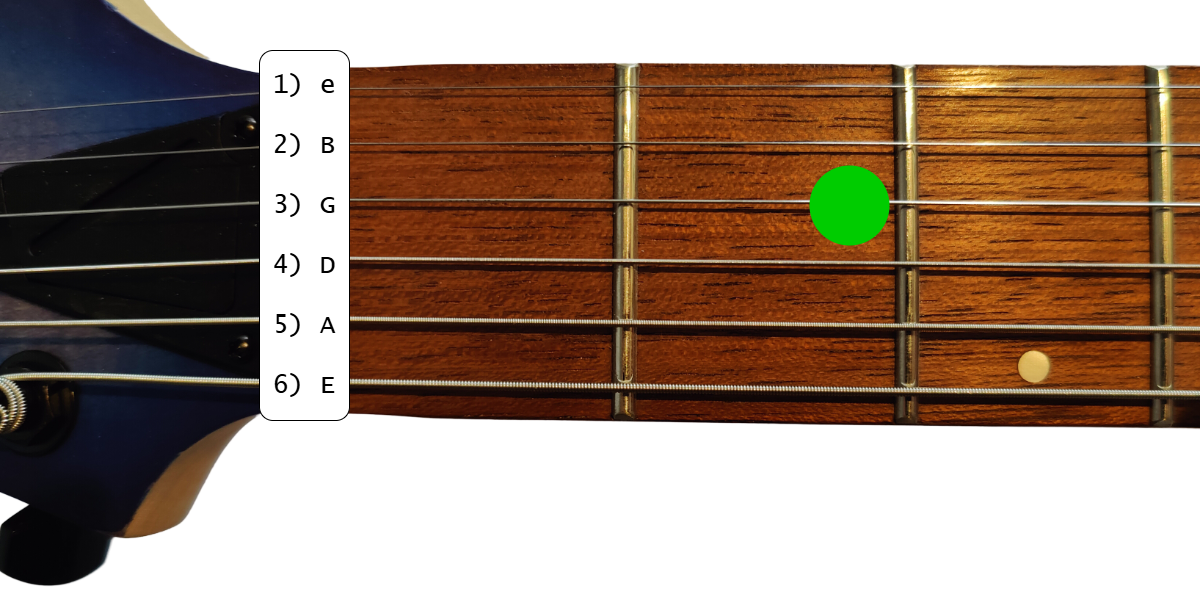
\includegraphics[width=\textwidth]{../../Images/guitar-neck-fretting.png}
    \captionof{figure}{The green dot in the finger placement for the 2nd fret on the 3rd string}
    \label{fig:guitar_string_fretting}
\end{minipage}

In music there are 12 different pitches before coming 'back around'. When you come back at the same note letter you are an octave higher. The 12 different notes are shown below.

\begin{table}[h]
\centering
\begin{NiceTabular}{*{12}{P{5mm}}}
\large{A} & \large{A\sharp} & \large{B} & \large{C} & \large{C\sharp} & \large{D} & \large{D\sharp} & \large{E} & \large{F} & \large{F\sharp} & \large{G} & \large{G\sharp}
\end{NiceTabular}
\end{table}

You may see that there are only \textbf{7} different letters and \textbf{5} letters with a \textbf{\sharp}. These $\sharp$ symbols are called \textbf{sharps}. On the fretboard a $\sharp$ means you move one fret up (to the body of the guitar).

In \autoref{fig:guitar_string_a_octave_single_string_sharps} you see a \textbf{music staff} with underneath it \textbf{tablature (TAB)}. In the next section we will learn to read the notes. For now you can try to read the tabs first to play the sequence.

Each line in the TAB section represents a guitar string, with the 6th (thickest) string on the bottom. The numbers indicate which fret should be pressed (a 0 means an open string). So the TAB in \autoref{fig:guitar_string_a_octave_single_string_sharps} says to first play an open A string, and then play each ascending fret up to the 12th fret.

\begin{figure}[h]
    \centering
    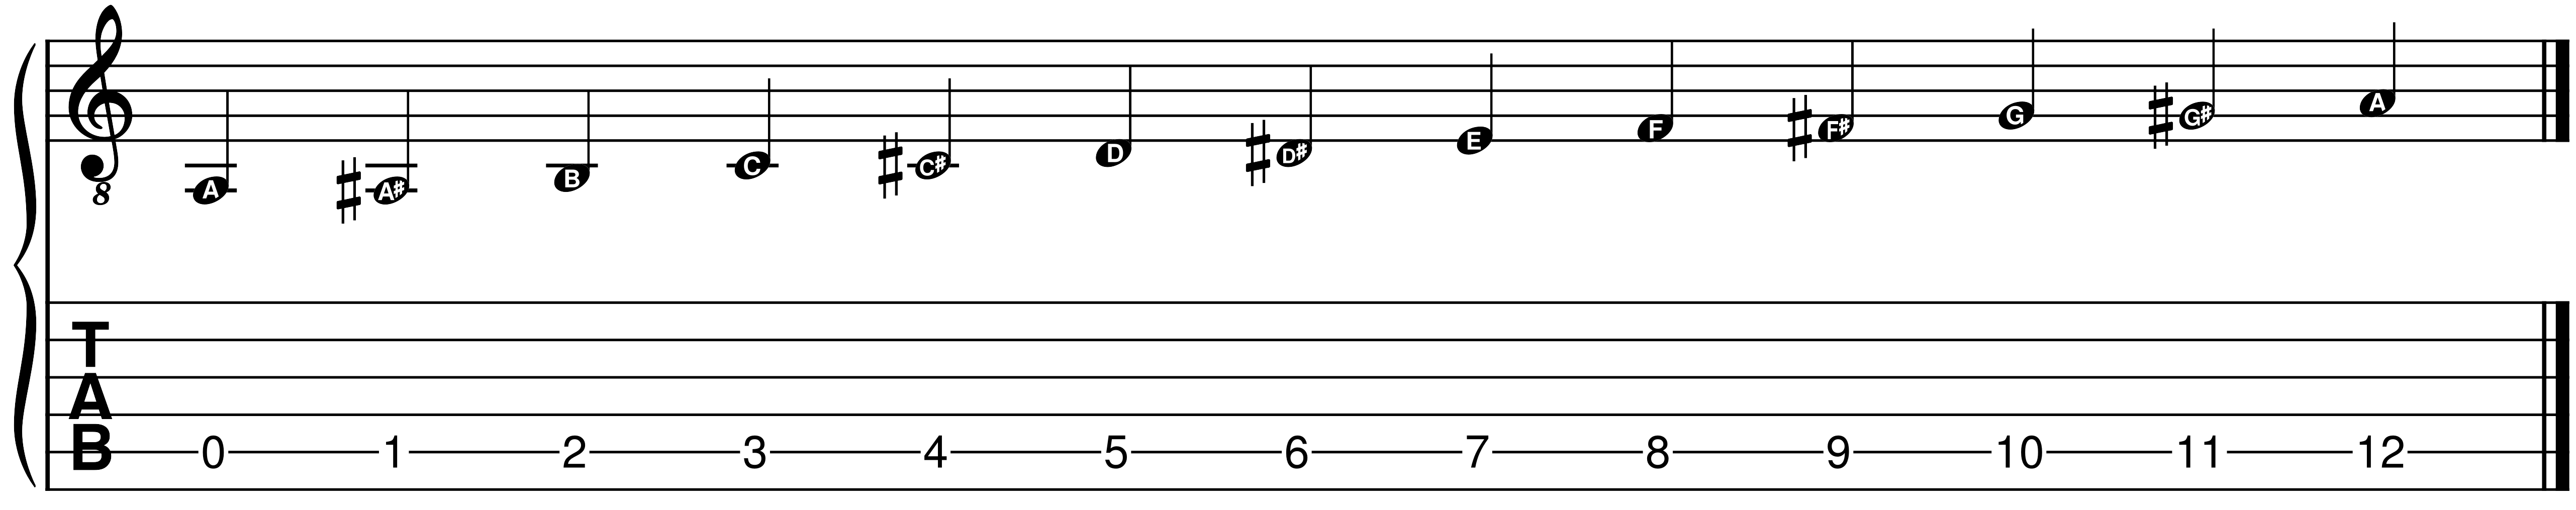
\includegraphics[width=\textwidth]{../../MuseScore/Guitar/PitchesSharpsSingleString.png}
    \caption{An octave from A to A on the 5th A string using sharps}
    \label{fig:guitar_string_a_octave_single_string_sharps}
\end{figure}

\newpage

Previously it was mentioned that the same pitch can be found on multiple strings. This is illustrated in \autoref{fig:guitar_string_a_octave_multi_string_sharps}. These are the name ascending notes/pitches as in \autoref{fig:guitar_string_a_octave_single_string_sharps}, but played on a different string.

This also indicates a big difference between tabs and notes. With notes, the expected sound (pitch) is described. You are free to determine where to play this on the fretboard. Tabs show one possible position to play the notes. You are of course still free to change the position as long as the resulting pitch is the same. But to do this you have to know where each note is on the fretboard.

\begin{figure}[h]
	\centering
	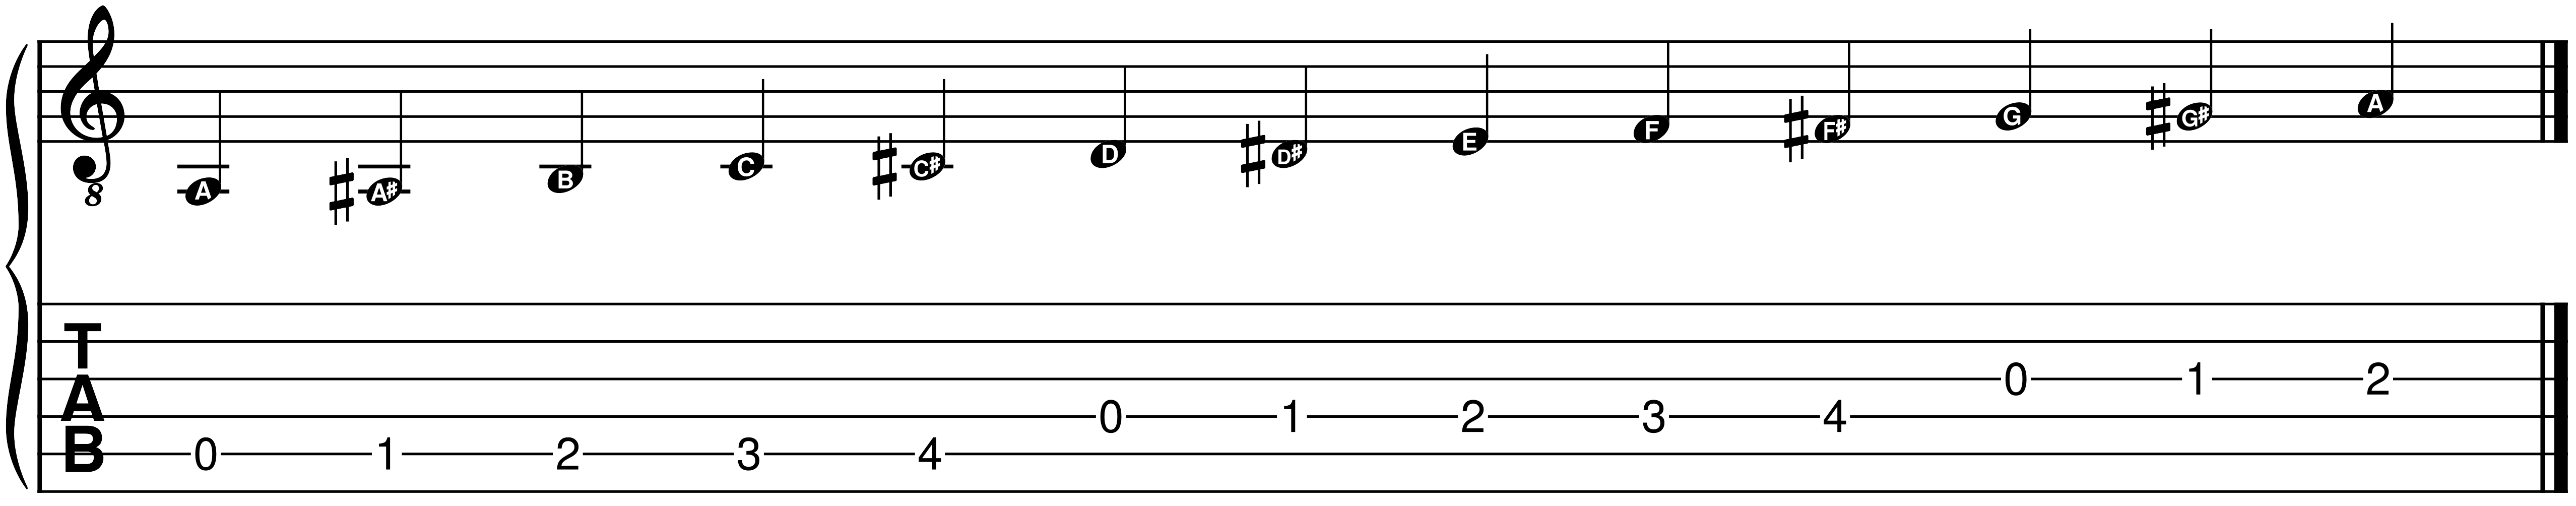
\includegraphics[width=\textwidth]{../../MuseScore/Guitar/PitchesSharpsMultiString.png}
	\caption{An octave from A to A on the multiple strings using sharps}
	\label{fig:guitar_string_a_octave_multi_string_sharps}
\end{figure}

Besides sharps there are also flats. A flat (\flat) means to go a halve tone (one fret) down. Rewriting \autoref{fig:guitar_string_a_octave_multi_string_sharps} with flats would look like \autoref{fig:guitar_string_a_octave_multi_string_flats}.

In \autoref{fig:guitar_string_a_octave_multi_string_flats} also a new symbol is shown. The natural (\natural). This means that the note on which a $\flat$ or $\sharp$ was placed, now is 'normal' again. Whenever a $\flat$ or $\sharp$ is added to a note, it remains valid for this note up to the end of the measure. What a 'measure' is will be explained later.

\begin{figure}[h]
	\centering
	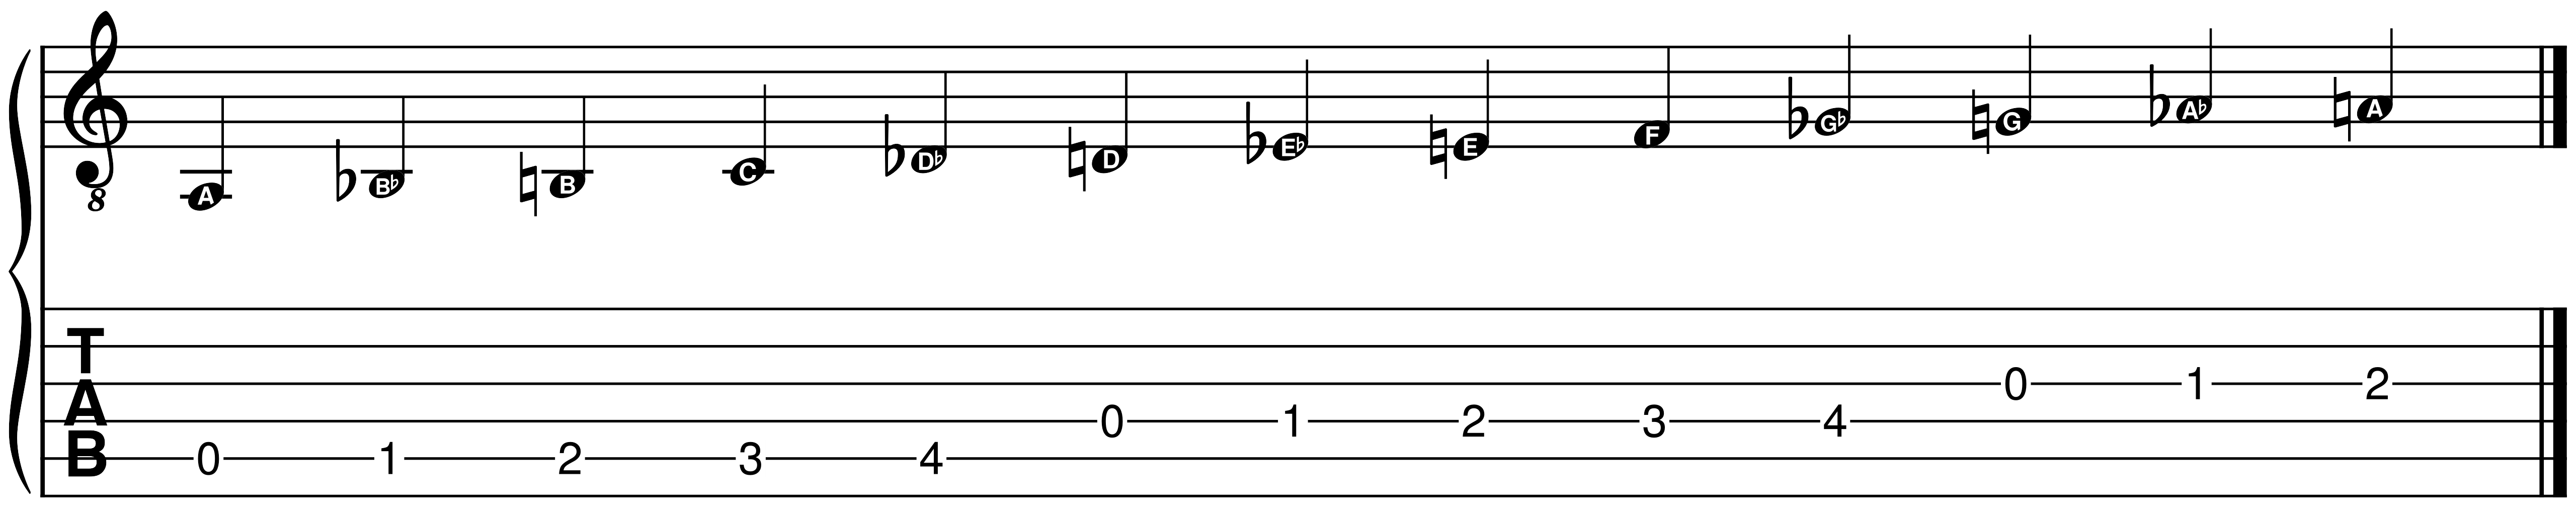
\includegraphics[width=\textwidth]{../../MuseScore/Guitar/PitchesFlatsMultiString.png}
	\caption{An octave from A to A on the multiple strings using flats and naturals}
	\label{fig:guitar_string_a_octave_multi_string_flats}
\end{figure}